\documentclass{INTERSPEECH2023}

\interspeechcameraready

\title{Better Music Demixing with the sliCQ Transform}
\name{Sevag Hanssian$^1$}
%The maximum number of authors in the author list is 20. If the number of contributing authors is more than this, they should be listed in a footnote or the acknowledgement section.
\address{$^1$Independent researcher (\url{sevag.xyz}), Montr{\'e}al, Canada}
\email{sevagh@protonmail.com}

\begin{document}

\maketitle
 
\begin{abstract}
% 1000 characters. ASCII characters only. No citations.
Music source separation, or music demixing, is the task of decomposing a song into its constituent sources, which are typically isolated instruments (e.g., drums, bass, and vocals). Open-Unmix (UMX), and the improved variant CrossNet-Open-Unmix (X-UMX), are high-performing models that use Short-Time Fourier Transform (STFT) as the representation of music signals, and apply masks to the magnitude STFT to separate mixed music into four sources: vocals, drums, bass, and other.

        The time-frequency uncertainty principle states that the STFT of a signal cannot be maximally precise in both time and frequency. The tradeoff in time-frequency resolution can significantly affect music demixing results. For the Cadenza Challenge in 2023, we submitted a model, xumx-sliCQ-V2,\footnote{\url{https://github.com/sevagh/xumx-sliCQ/tree/v2}} which replaces the STFT with the sliCQT, a time-frequency transform with varying time-frequency resolution. Our system achieved an SDR score of 4.4 dB on the MUSDB18-HQ test set. 
\end{abstract}
\noindent\textbf{Index Terms}: music source separation, music demixing, deep neural networks, time-frequency resolution, MUSDB18-HQ

\section{Introduction}

The STFT is computed by applying the Discrete Fourier Transform on fixed-size windows of the input signal. From both auditory and musical motivations, variable-size windows are preferred, with long windows in low-frequency regions to capture detailed harmonic information with a high frequency resolution, and short windows in high-frequency regions to capture transients with a high time resolution \cite{doerflerphd}. The sliCQ Transform (sliCQT) \cite{slicq} is a time-frequency transform with complex Fourier coefficients and perfect inverse that uses varying windows to achieve nonlinear time or frequency resolution. An example application of the sliCQT is an invertible Constant-Q Transform (CQT) \cite{jbrown}.

\section{Methodology}

From the guidelines of the Cadenza challenge and to ensure reproducibility, we only relied on the standard and widely-available MUSDB18-HQ dataset \cite{musdb18hq} for training and evaluation of xumx-sliCQ-V2.

In xumx-sliCQ-V2, we kept the same sliCQT parameters from the older variant, xumx-sliCQ \cite{hanssian21}. The sliCQT parameters are 262 bins on the Bark scale between 32.9--22050 Hz, chosen in a random parameter search to maximize the mix-phase or noisy-phase oracle \cite{hanssian21}. STFT and sliCQT spectrograms of a glockenspiel signal are shown in Figure \ref{fig:spectrograms}.

The STFT outputs a single time-frequency matrix where all of the frequency bins are spaced uniformly apart and have the same time resolution. The sliCQT groups frequency bins, which may be nonuniformly spaced, in a ragged list of time-frequency matrices, where each matrix contains frequency bins that share the same time resolution. In xumx-sliCQ-V2, convolutional layers were applied separately to each time-frequency matrix, shown in Figure \ref{fig:ragged}.

We made three significant changes to the older system, xumx-sliCQ, which account for the improved performance of xumx-sliCQ-V2.

\balance
\begin{figure*}[h]
  \begin{minipage}{\linewidth}
        \centering
	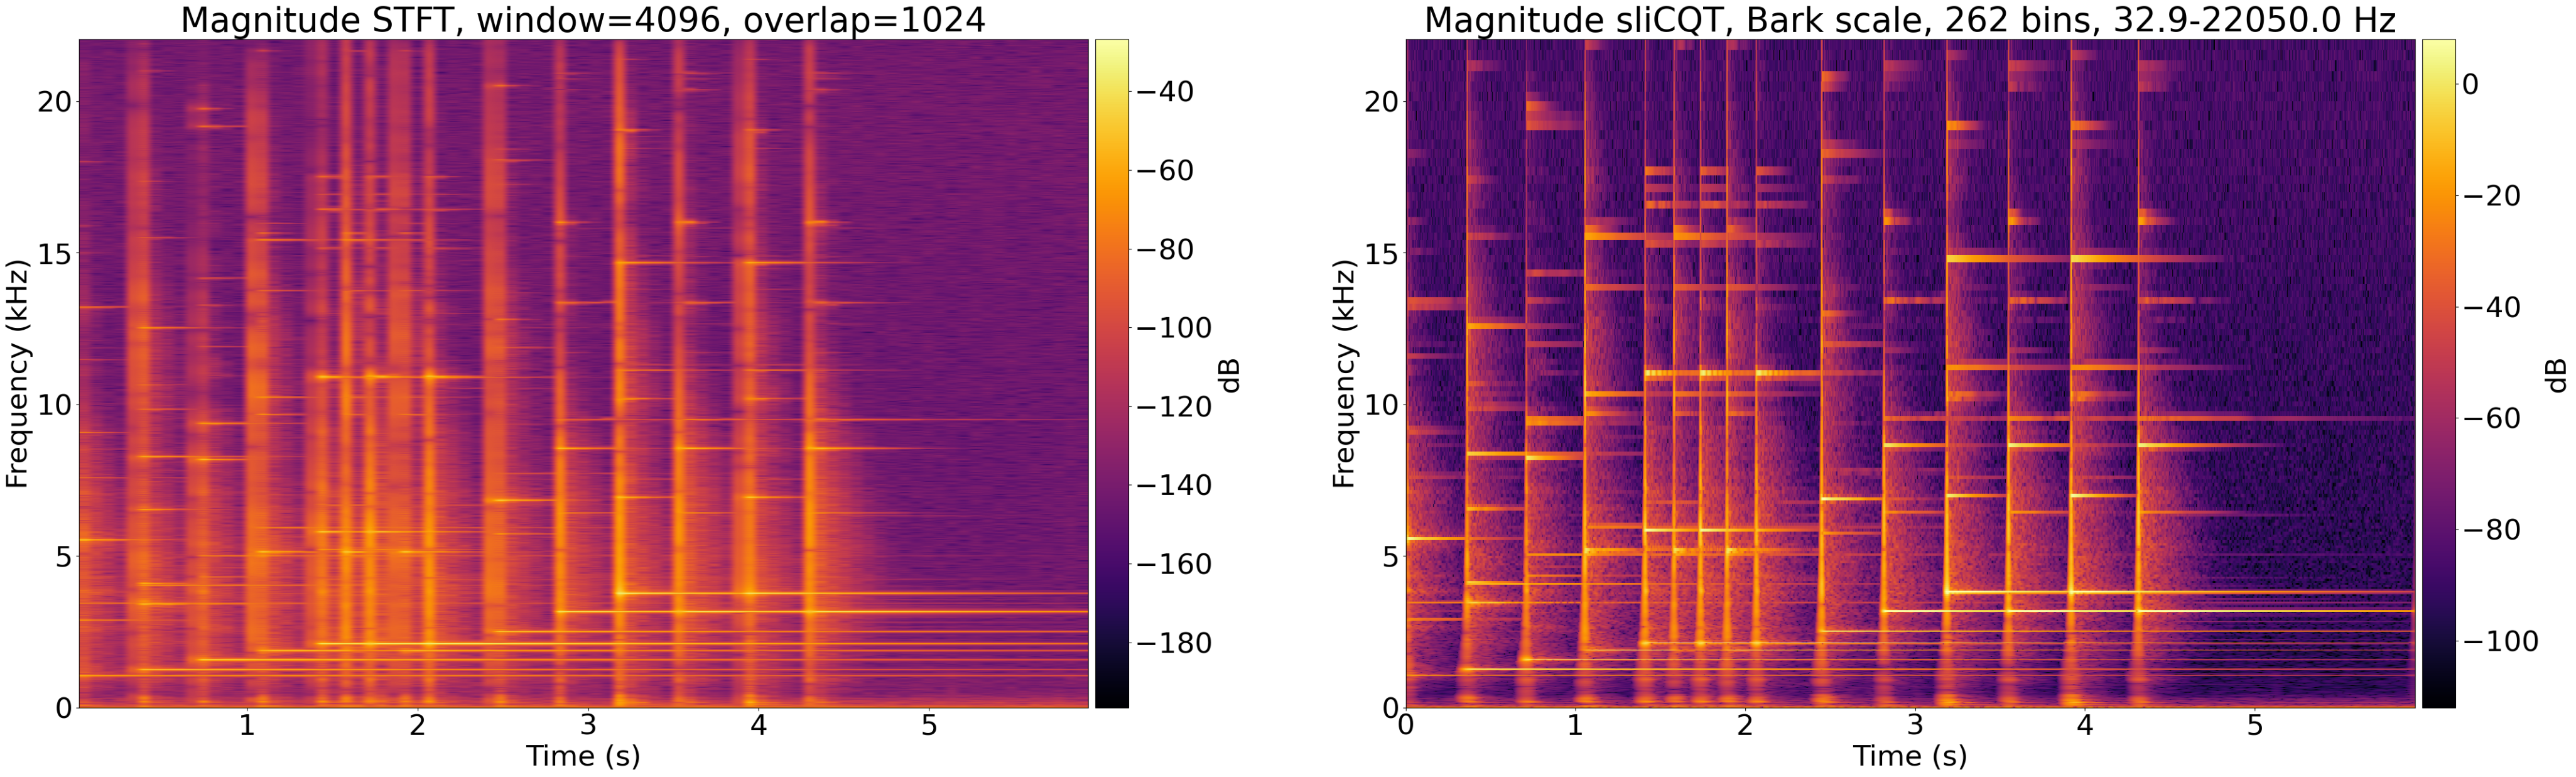
\includegraphics[width=0.65\textwidth]{./spectrograms_comparison.png}
	\caption{STFT and sliCQT spectrograms of the musical glockenspiel signal}
	\label{fig:spectrograms}
  \end{minipage}

  \begin{minipage}{\linewidth}
        \centering
	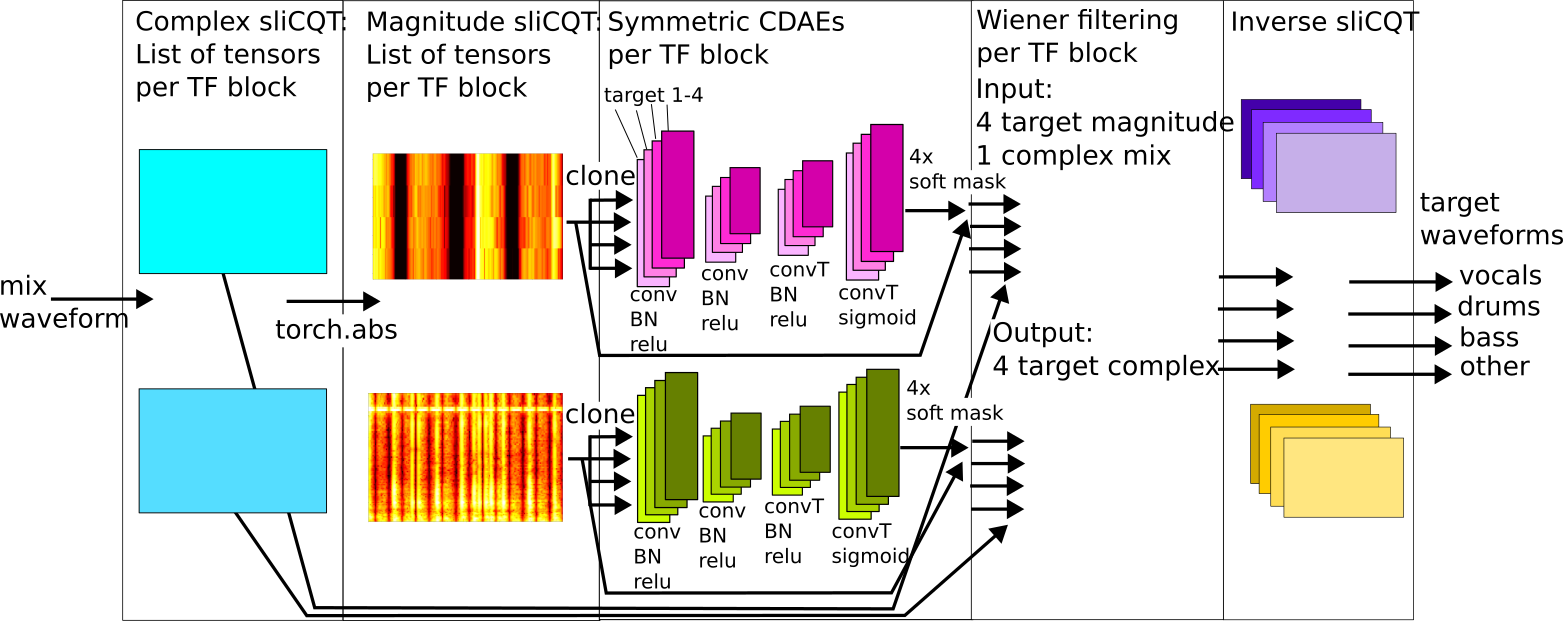
\includegraphics[width=0.65\textwidth]{./xumx_slicq_pertarget.png}
	\caption{Convolutional denoising autoencoders (CDAE) applied to the ragged sliCQT}
	\label{fig:ragged}
  \end{minipage}

  \begin{minipage}{\linewidth}
        \centering
        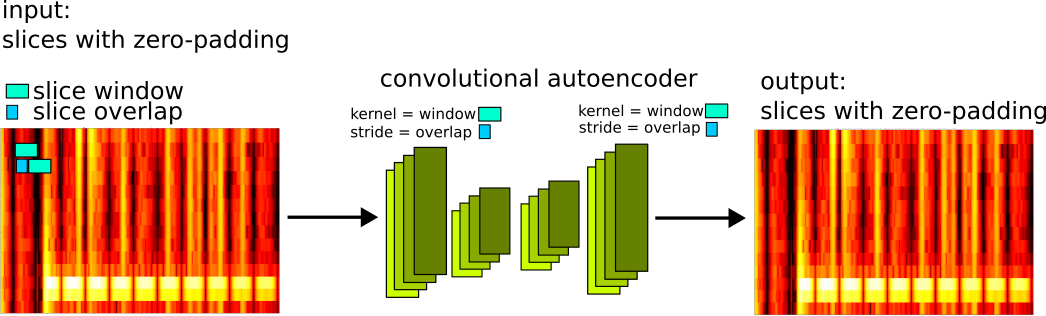
\includegraphics[width=0.45\textwidth]{./overlap.png}
	\caption{Incorporating slice zero-padding into the convolutional layers}
	\label{fig:overlap}
  \end{minipage}
\end{figure*}

\subsection{Improved overlap-add}

The sliCQT subdivides the input signal into ``slices'' of length $N$ that are ``symmetrically zero-padded to length $2N$'' \cite[10]{slicq}. To create a spectrogram, adjacent slices need to be 50\% overlap-added with each other, with no inverse operation. In xumx-sliCQ-V2, we incorporated the slice size in the kernel and stride of the first convolution layer and last transpose convolution layer to avoid the non-invertible overlap-add procedure, shown in Figure \ref{fig:overlap}.

\subsection{Differentiable Wiener filtering and complex MSE}

In xumx-sliCQ, the mean-squared error (MSE) loss function is applied to the magnitude spectrogram estimates of the neural network. The post-processing Wiener filtering step is then used to further improve the separation results and create the estimated complex spectrograms. Danna-Sep \cite{yu2021dannasep}, a winning system from MDX 21, incorporated the Wiener filtering step into the neural network to output complex spectrograms, and used the complex mean-squared error as the loss function. We did the same in xumx-sliCQ-V2.

\subsection{Mask-sum loss}

The final activation layer of xumx-sliCQ-V2 is the sigmoid function ($\in [0.0, 1.0]$), to apply as a soft mask (or ratio mask) to the magnitude spectrogram of the mix. An underlying simplifying assumption in music demixing is that the mix is a linear sum of the sources. Therefore, the sum of the four target masks should be exactly equal to one, shown in Equation \eqref{eq:linmix}. In xumx-sliCQ-V2, we introduce an additional loss term called the ``mask-sum loss'' which computes the MSE of the sum of the estimated masks with the expected total mask of ones.

\begin{align}
        & x_{\text{mix}} = x_{\text{v}} + x_{\text{d}} + x_{\text{b}} + x_{\text{o}} \nonumber \\
        & |X|_{\text{mix}} = M_{\text{v}}|X|_{\text{mix}} + M_{\text{d}}|X|_{\text{mix}} + M_{\text{b}}|X|_{\text{mix}} + M_{\text{o}}|X|_{\text{mix}} \nonumber \\
        & 1 = M_{\text{v}} + M_{\text{d}} + M_{\text{b}} + M_{\text{o}} \label{eq:linmix}
\end{align}

\section{Results}

Our model, xumx-sliCQ-V2, was trained on MUSDB18-HQ. On the test set, xumx-sliCQ-V2 achieved a total SDR of 4.4 dB versus the 4.64 dB of UMX and 5.54 dB of X-UMX, performing worse than the original STFT-based models, but better than the first xumx-sliCQ which scored 3.6 dB.

\section{Discussion}

The Cadenza Challenge Task 1 applies further processing on top of the VDBO demixing system, and the final evaluation uses the HAAQI metric. We chose to focus only on the VDBO music demixing problem, and used BSS metrics to measure the improvement of xumx-sliCQ-V2 over xumx-sliCQ.

We believe that the mask-sum loss term of xumx-sliCQ-V2 to enforce the linear additive mixture assumption can be generally applied to any system based on spectrogram-masking and potentially improve their results.

\section{Conclusion}

We presented xumx-sliCQ-V2, an improved variant of xumx-sliCQ, which replaces the STFT of X-UMX with a Bark-scale sliCQT, a nonuniform time-frequency transform whose characteristics more closely map to the human auditory system. The total SDR went from 3.6 dB to 4.4 dB, demonstrating significantly improved music demixing results from the changes in xumx-sliCQ-V2.

\bibliographystyle{IEEEtran}
\bibliography{mybib}

\end{document}
